\index{instructions}

\begin{figure}[hbt]
\centering
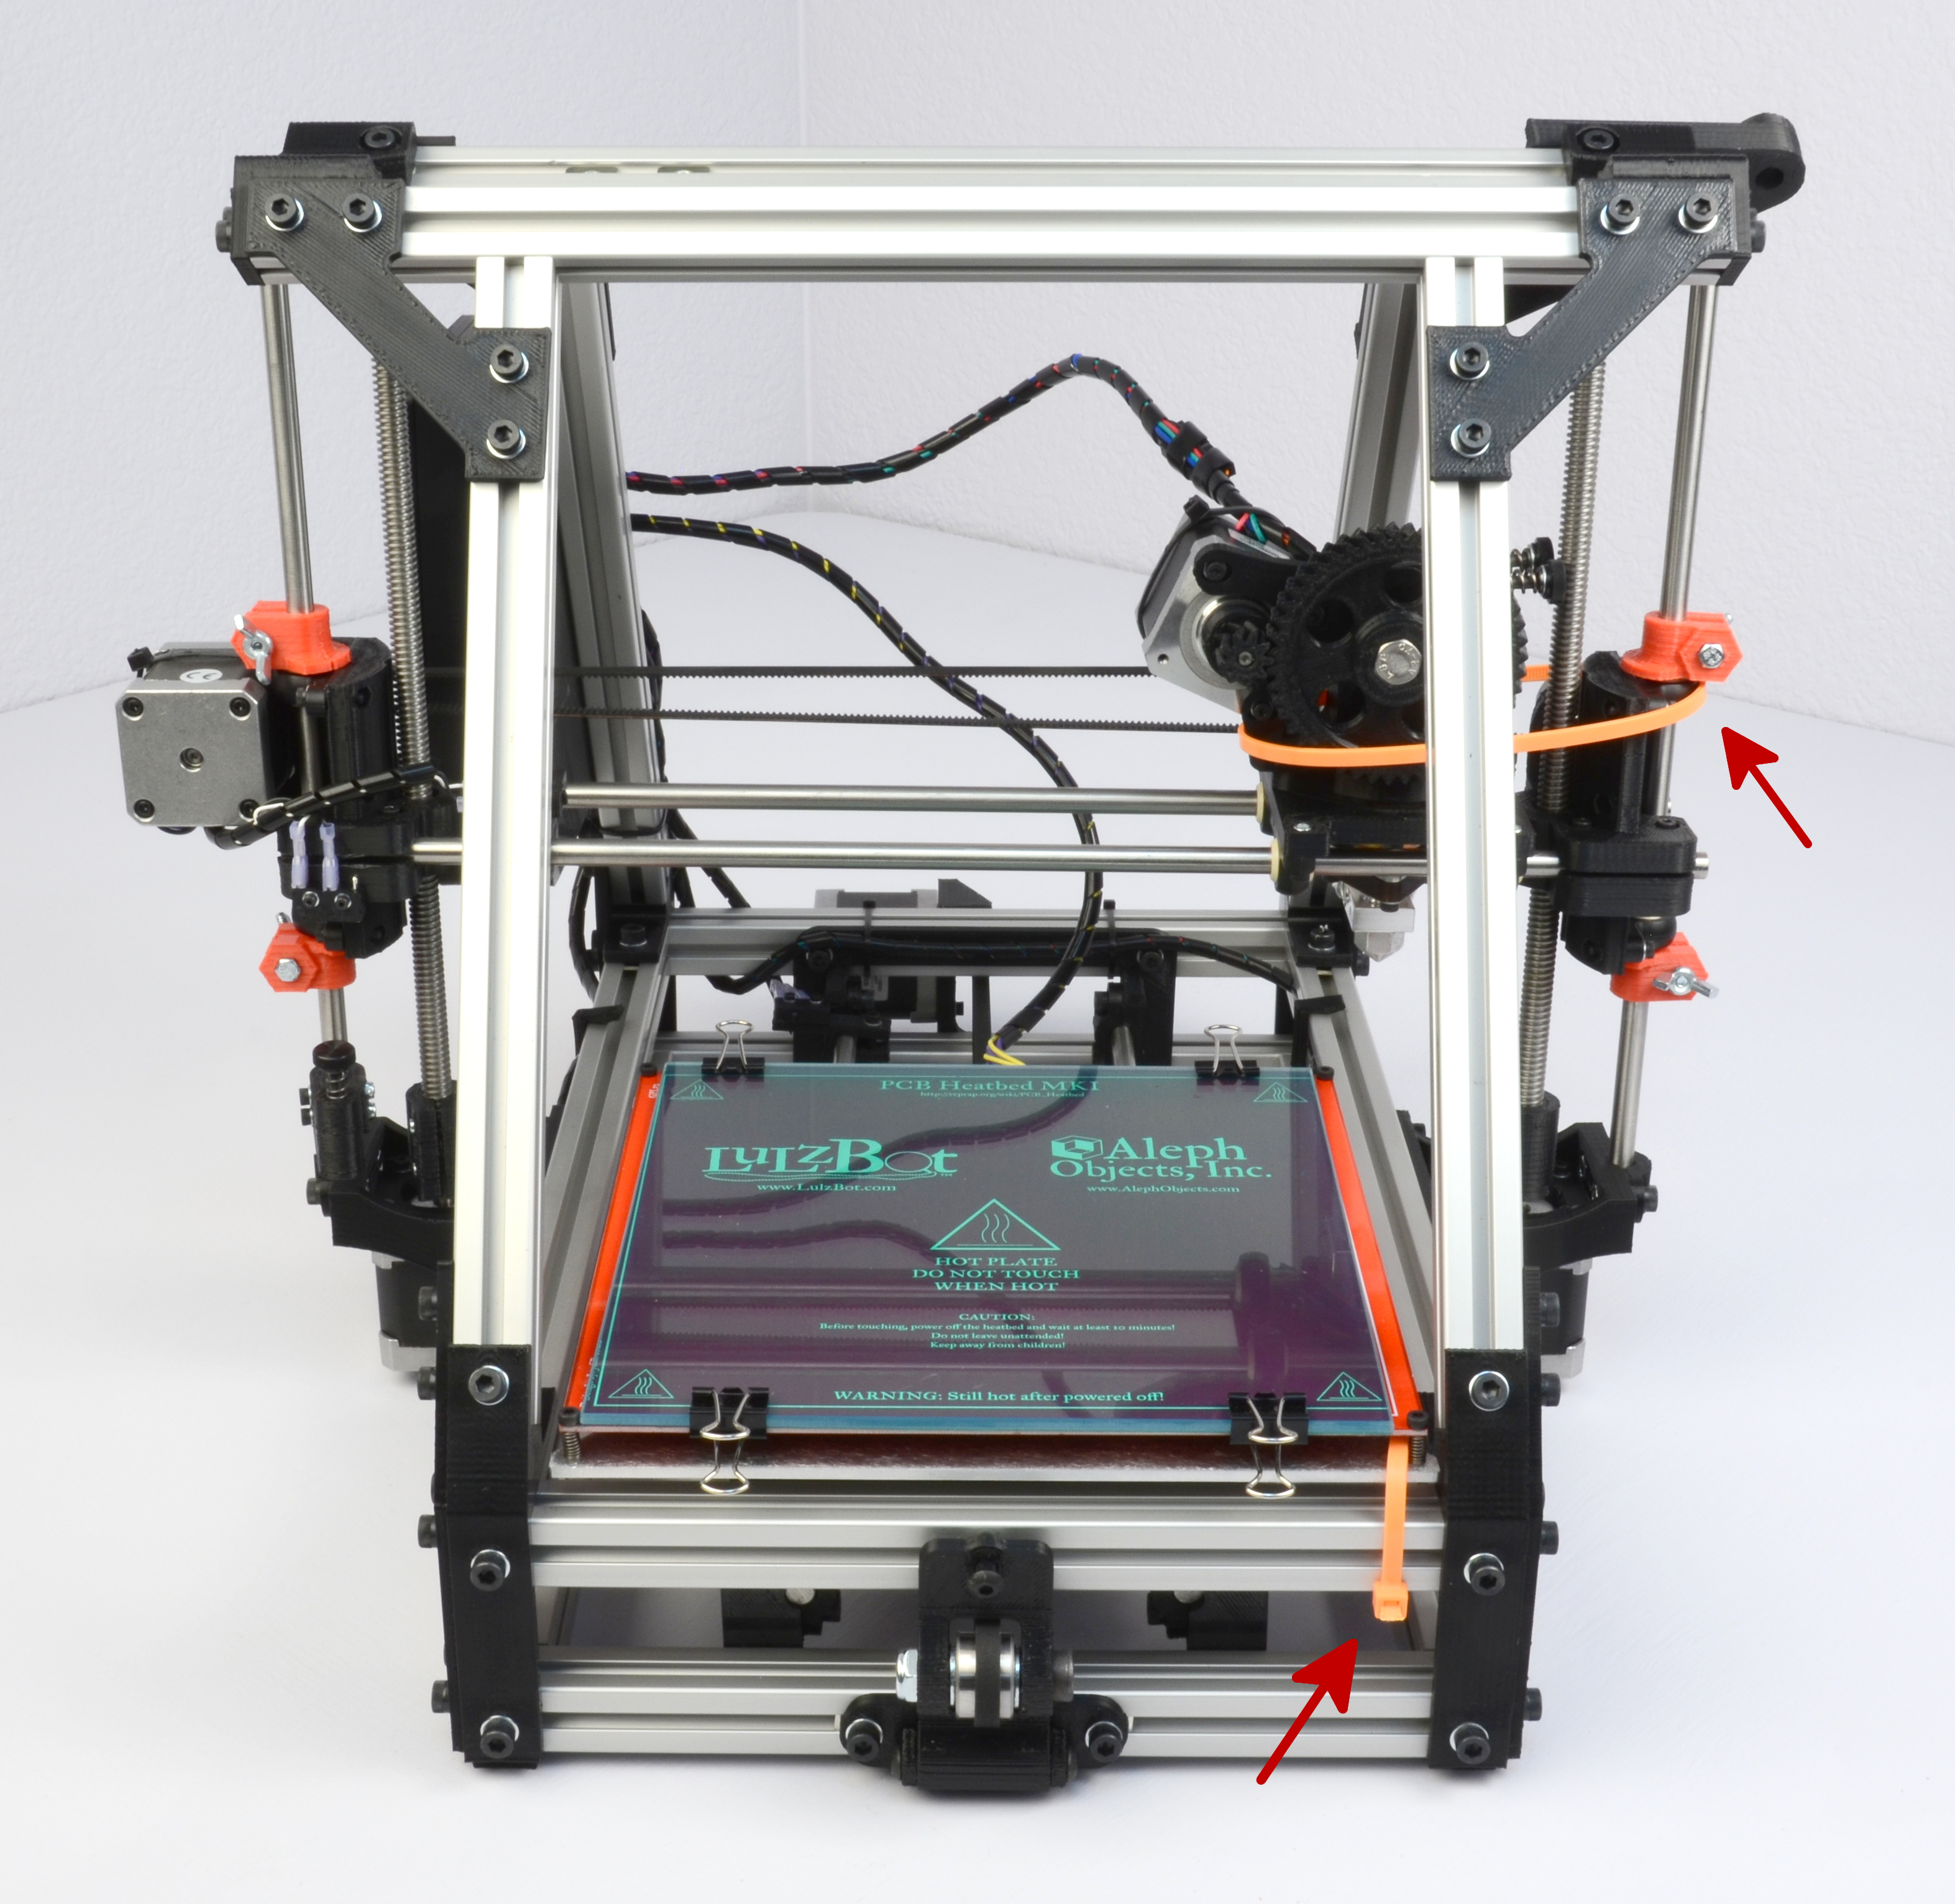
\includegraphics[keepaspectratio=true,angle=0,height=0.4\textheight,width=1.0\textwidth]{zip_ties.jpg}
\caption{Orange Zip Ties}
\label{fig:zip_ties}
\end{figure}

\begin{enumerate}
\item Remove the plastic bag containing instructions, cords, and small parts.

\index{foam padding}
\item Remove the top foam padding. 

\index{filament spool}
\index{filament guide}
\item Slowly remove the two smaller foam pads. One of these pads will contain the plastic filament spool and plastic filament guide. The other pad will contain the 5lb coil of ABS plastic filament. With the two small foam pads remove and set aside these items.

\index{power supply}
\index{tool bag}
\item Remove the white power supply box and the black tool bag. These items are along opposite sides of the printer.

\item Grab the top of the wrapped printer on the top center where you will feel two lengths of square aluminum tubing. Holding the top two tubes, SLOWLY pull the printer upwards out of the box. The two large side foam pads should fall off when the printer is out of the box.

\item Set you printer on a stable level surface.

\item Gently unwrap the pink ESD plastic covering the printer. Remove the rolled sheet of PET tape from below the print bed. Gently lift the printer to slide the plastic wrapping from under the printer. 

\item Find the item list attached to the plastic bag of parts. Before you move on to setting up your printer make sure all of the items on the list are in your package.

\item Using scissors or wire cutters, cut and remove the two ORANGE plastic zip ties
(Fig. \ref{fig:zip_ties}, page \pageref{fig:zip_ties})
. One zip tie is located on the bottom front of the printer on the print bed. The other zip tie is wrapped around the extruder carriage and X axis. Make sure to not cut any of the surrounding wires or belts.

\begin{figure}[hbt]
\centering
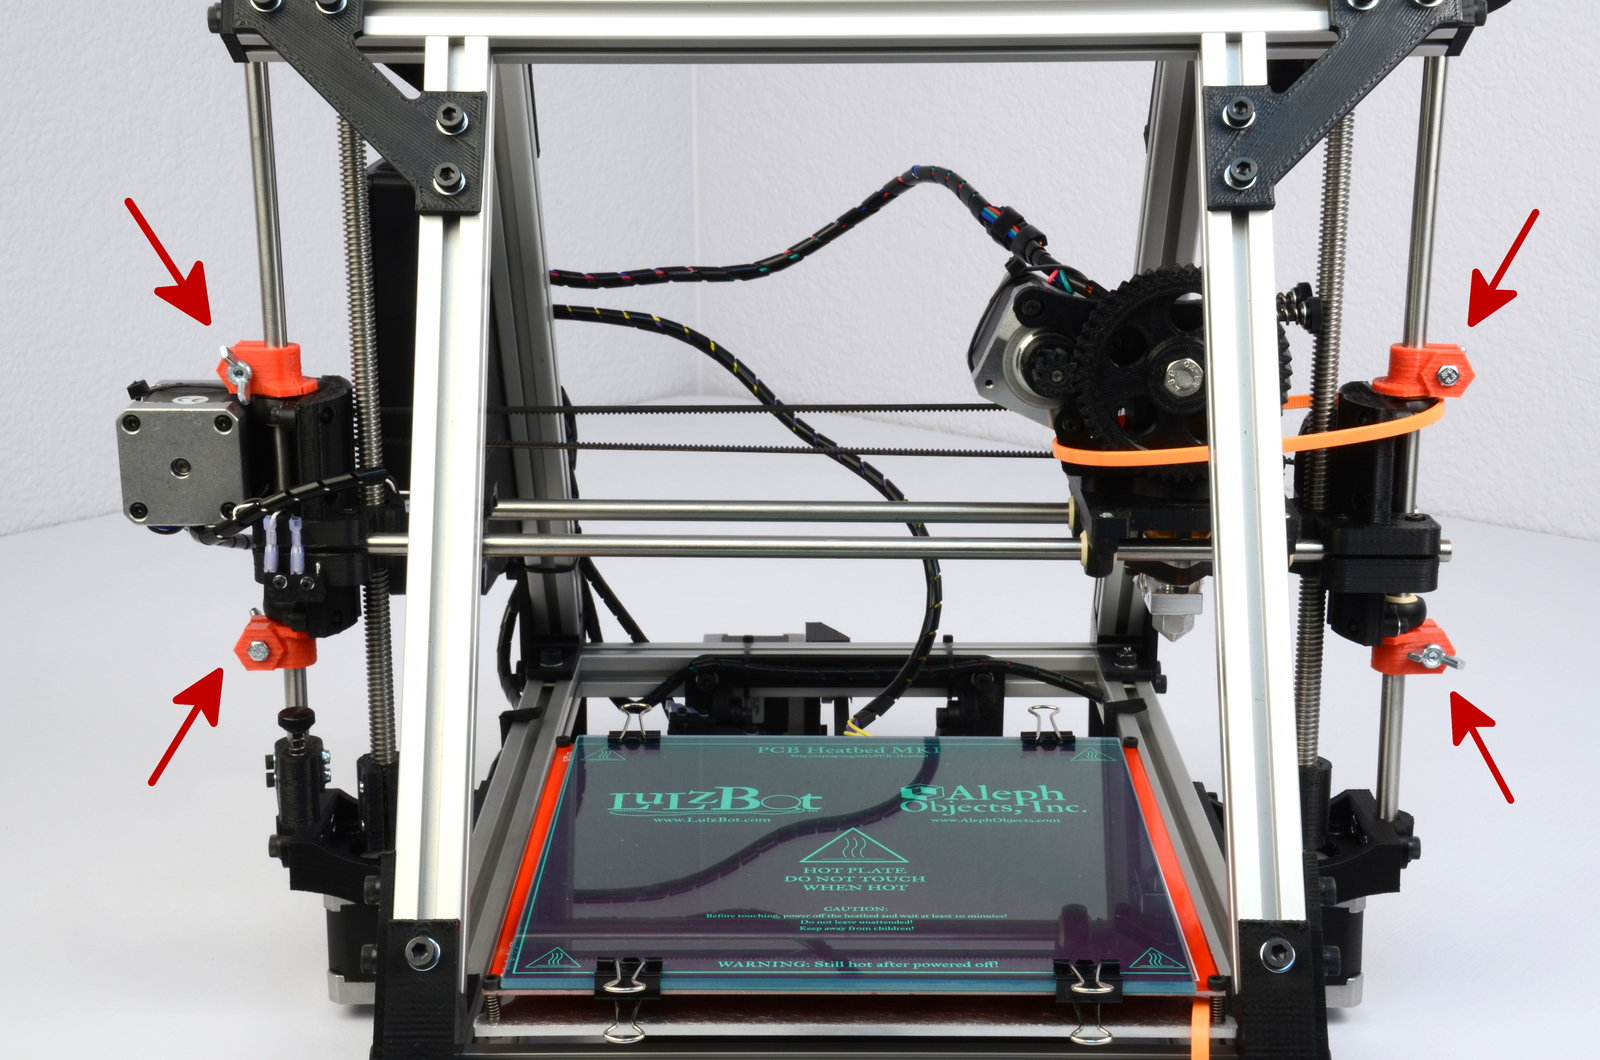
\includegraphics[keepaspectratio=true,angle=0,height=0.4\textheight,width=1.0\textwidth]{shipping_clamps.jpg}
\caption{Red Shipping Clamps}
\label{fig:shipping_clamps}
\end{figure}

\index{shipping clamps}
\index{x-end motor mount}
\index{idler}
\item Remove the four red shipping clamps above and below the x-end motor mount and idler
(Fig. \ref{fig:shipping_clamps}, page \pageref{fig:shipping_clamps}).

\item Loosen and remove the wing nut and screw on each of the four clamps. Remove each of the four clamps by popping them off of the smooth rod. Use a screwdriver or wrench to pry open and remove the clamps if you have trouble removing them by hand (Fig. \ref{fig:shipping_clamps_pry}, page \pageref{fig:shipping_clamps_pry}). Keep the clamps and hardware for future use if you need to ship or transport your printer.

\begin{figure}[hbt]
\centering
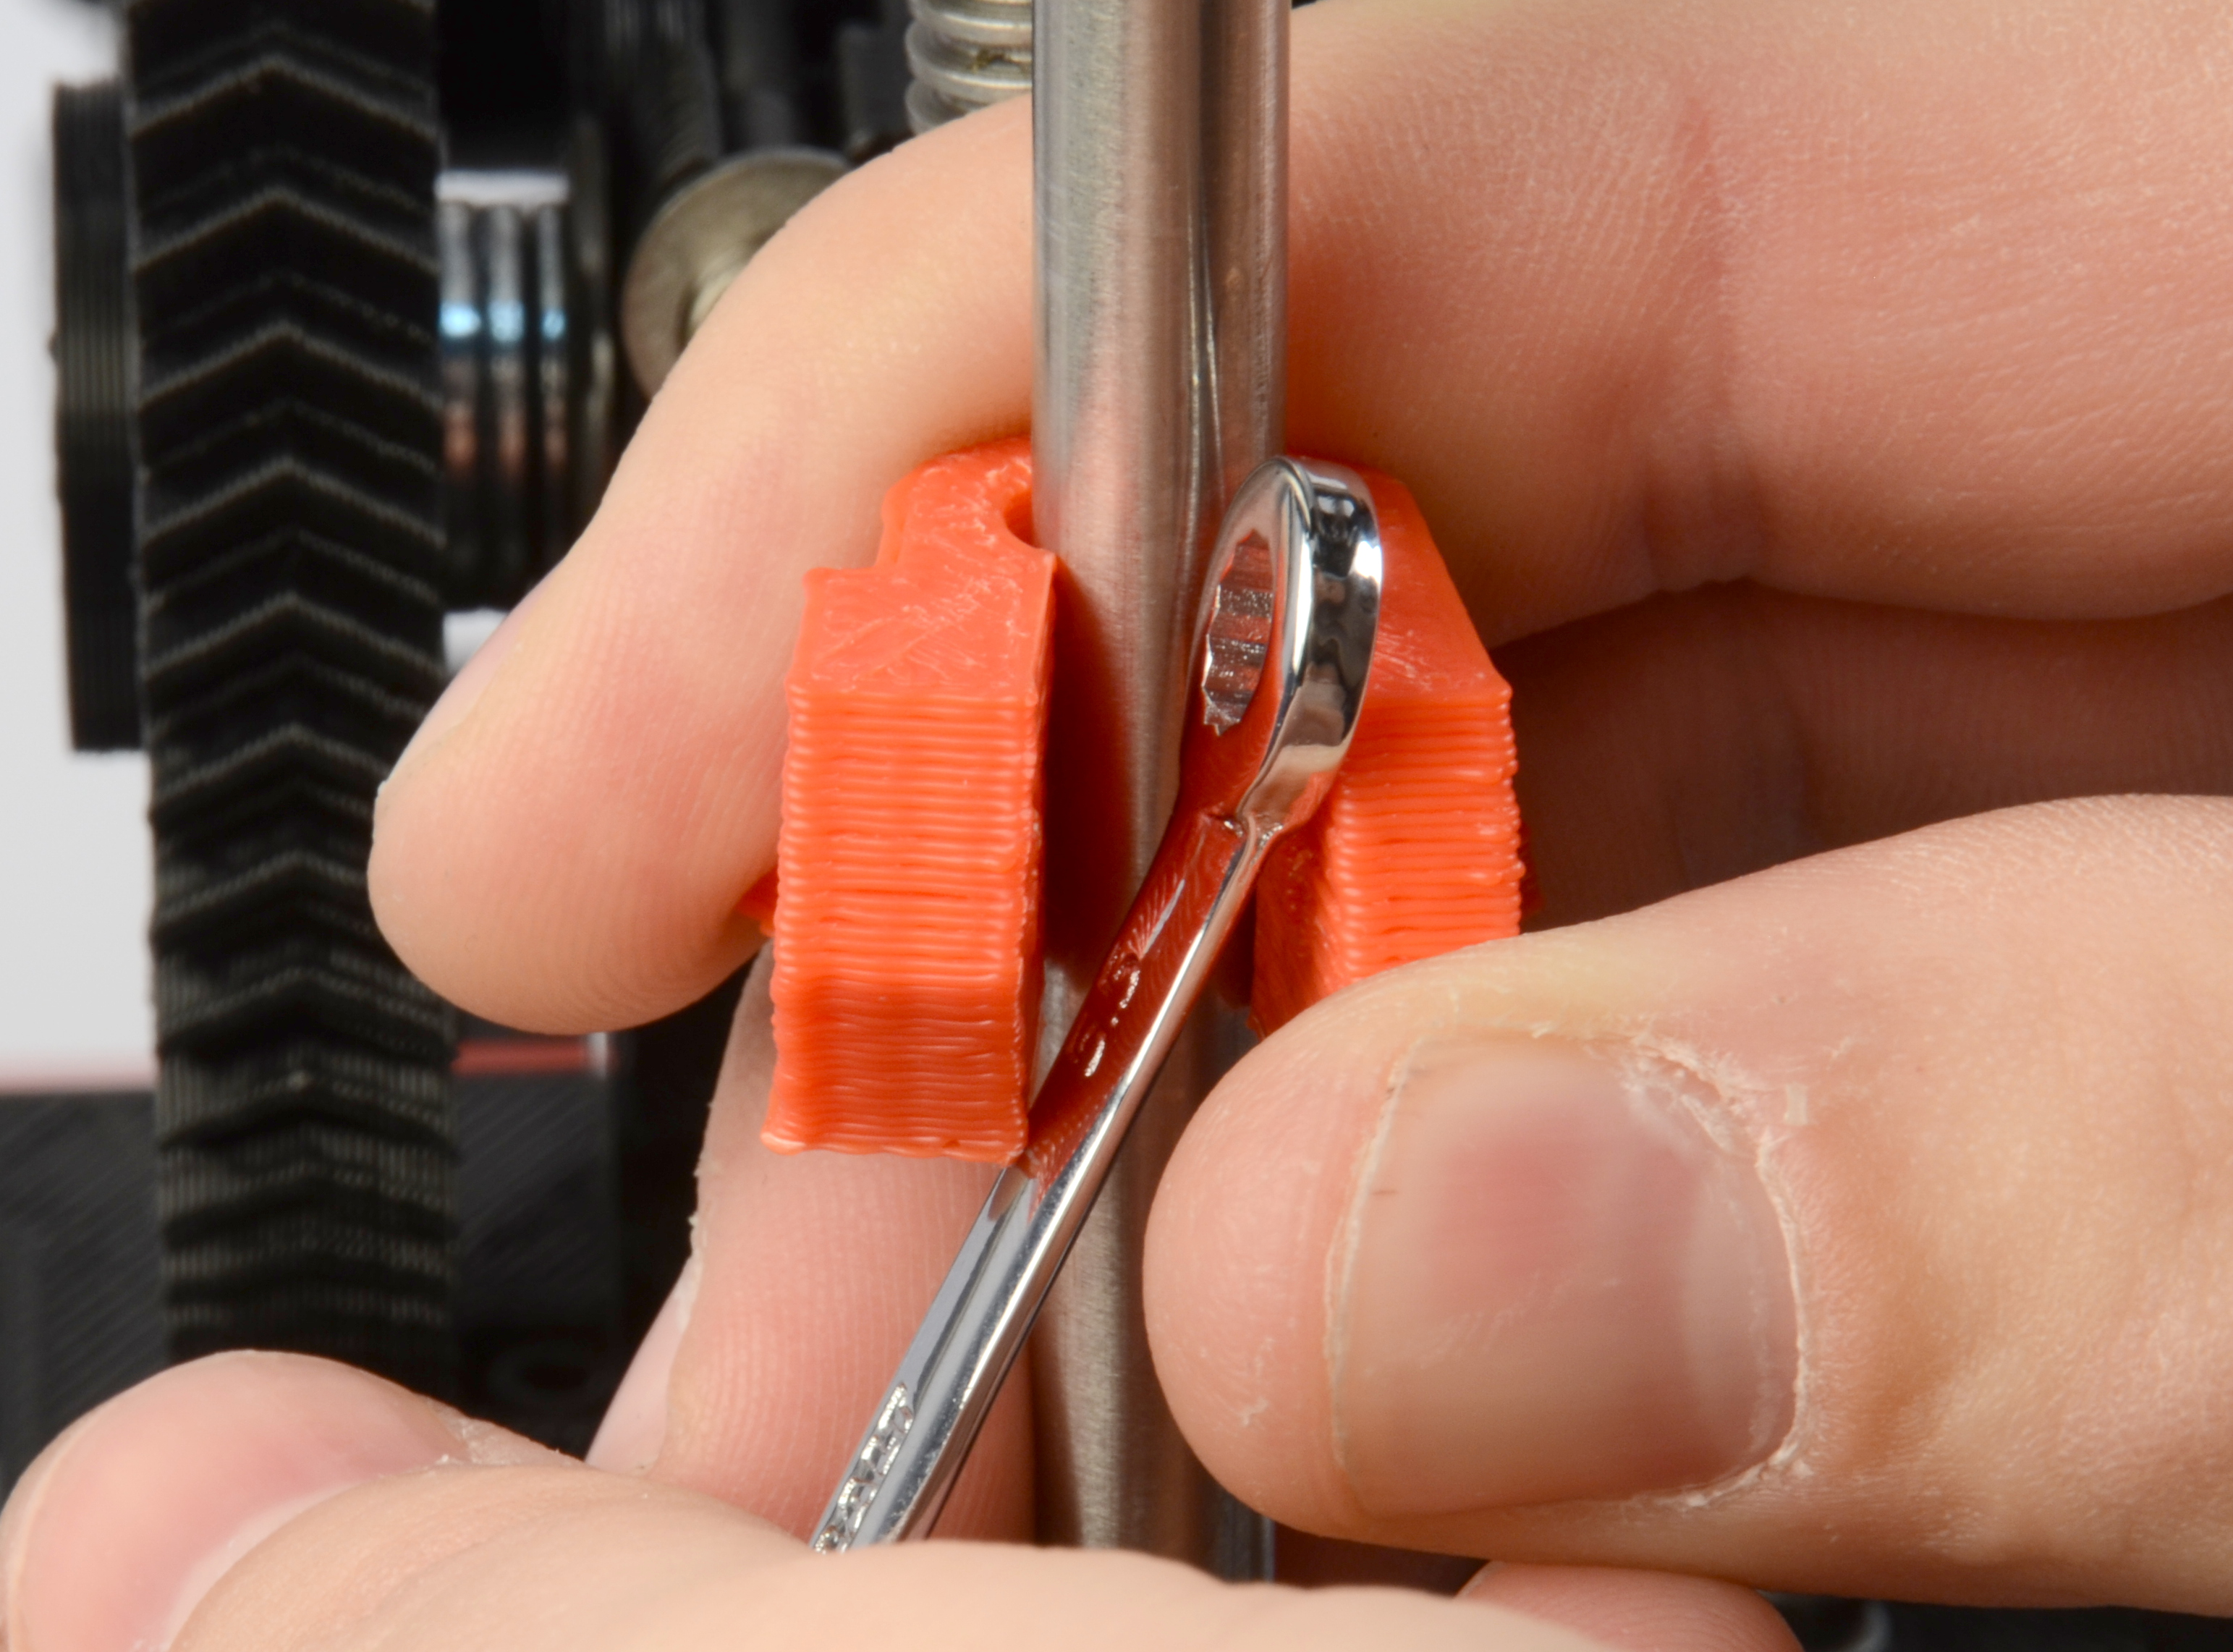
\includegraphics[keepaspectratio=true,angle=0,height=0.4\textheight,width=1.0\textwidth]{shipping_clamps_pry.jpg}
\caption{Using a wrench to pry off the shipping clamps}
\label{fig:shipping_clamps_pry}
\end{figure}

\index{blue tape}
\index{PET sheet}
\item Remove the blue tape from the sides of the print surface. Make sure to not remove the green PET tape on the glass print surface. The PET tape helps keep the print attached to the print surface during printing.

\end{enumerate}
